\documentclass[../main.tex]{subfiles}
\begin{document}
\chapter{Uniform Convergence}
\section{Pointwise Convergence}
\subsection{Definition}
Consider some set $E \subseteq \R$ and a sequence of functions $f_n: E \to \R$.
What could it mean for the sequence $(f_n)_{n \in \N}$ to converge?

The most basic thing we can do is to consider \textit{pointwise} convergence.
\begin{definition}[Convergence at a point]
  We say that a sequence of functions $(f_n)_{n \in \N}$ convergences at a point $x \in E$ if the real sequence $(f_n(x))_{n \in \N}$ converges.
\end{definition}
\begin{definition}[Pointwise Convergence]
  We say that a sequence of functions $(f_n)_{n \in \N}$ \textit{converges pointwise} if it converges at all points $x \in E$.
  Since it converges at each point, we say that it \textit{converges pointwise} to a function $f$ defined as: \label{pointwiseDef}
  \[
    f(x) = \lim_{n \to \infty} f_n(x)
  \]
  We then write that $f_n \to f$ pointwise on $E$.
\end{definition}
\begin{remark}
  $f$ as defined above is well defined function due to the uniqueness of limits.
\end{remark}
\subsection{Problems with Pointwise Convergence}
Ideally, we would like to use properties such as continuity, differentiability, integrability from the functions $f_n$ in the sequence, for this limit function $f$.
However the notion of pointwise convergence is not strong enough to make such conclusions.
\begin{example}[Continuity is not preserved]
  Let $E = [-1, 1]$ and define the series of continuous functions $f_n: E \to \R$ by:
  \[
    f_n: E \to \R,\ x \mapsto x^{\frac{1}{2n + 1}}
  \]
  This is pointwise convergent on $E$ with limit:
  \[
    f(x) = \begin{cases}
    1 & \text{ if } x > 0 \\
    0 & \text{ if } x = 0 \\
    -1 & \text{ if } x < 0
    \end{cases}
  \]
  This is discontinuous at $x = 0$ and so continuity is not preserved under pointwise convergence.
\end{example}
\begin{example}[Integrability is not preserved]
  In IA Analysis I, we saw that the Dirichlet function $1_\Q$ is not integrable on $[0, 1]$.
  We would like to construct a sequence of integrable functions $f_n$ such that $f_n \to 1_\Q$ pointwise on $[0, 1]$.

  Let $q_1, q_2, \ldots$ be an enumeration of $\Q \cap [0, 1]$ and define the sequence of functions by:
  \[
    f_n: [0, 1] \to \R,\ x \mapsto \begin{cases}
    1 & \text{ if } x \in \{q_1, \ldots, q_n\} \\
    0 & \text{ otherwise }
    \end{cases}
  \]
  For all $n \in \N$, $f_n$ is continuous except at some finite set of points $\{q_1, \ldots, q_n\}$ and so from IA Analysis I, we know that $f_n$ is integrable for all $n$.

  Clearly $f_n \to 1_\Q$ pointwise on $[0, 1]$, but $1_\Q$ \textbf{not} integrable and so integrability is not preserved under pointwise convergence.
\end{example}
If we have a sequence of functions $f_n$ which are all integrable and we assume that they indeed convergence pointwise to an integrable function $f$, does it follow that values of the integrals of $f_n$ converges to the value of the integral of $f$.
\begin{example}[Values of integrals are not preserved]
   Define the sequence of functions:
  \[
    f_n: [0, 2] \to \R,\ x \mapsto \begin{cases}
    n^2 x & \text{ if } x \in \left[0, \frac{1}{n}\right] \\
    n^2\left(\frac{2}{n} - x\right) & \text{ if } x \in \left[\frac{1}{n}, \frac{2}{n}\right] \\
    0 & \text{ otherwise }
    \end{cases}
  \]
  That is, the graph of $f_n$ is a triangle with vertices at $(0, 0)$, $(2/n, 0)$ and $(1/n, n)$.
  For $n \in \{1, \ldots, 5\}$ this looks like:
  \begin{center}
  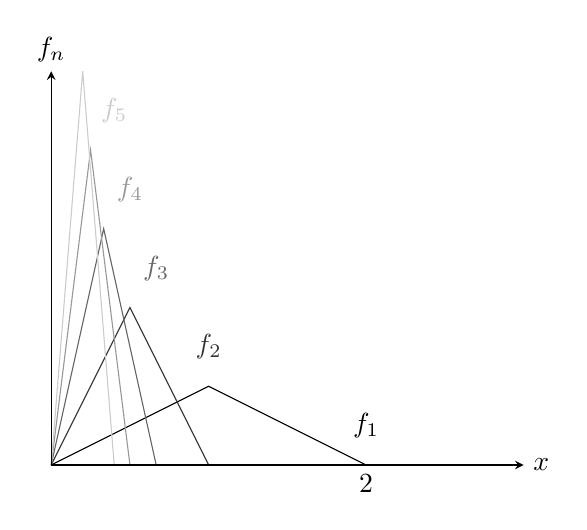
\begin{tikzpicture}[>=stealth]
    \foreach \n/\o in {1/100, 2/80, 3/60, 4/40, 5/20} {
      \begin{scope}[black!\o]
        \draw (0, 0) -- (2/\n, \n) -- (4/\n, 0);
        \node at (4/\n, \n - 0.5) {$f_\n$};
      \end{scope}
    }

    \draw[->] (0, 0) -- (0, 5) node[above] {$f_n$};
    \draw[->] (0, 0) -- (6, 0) node[right] {$x$};
    \node[below] at (4, 0) {2};
  \end{tikzpicture}
  \end{center}
  For each $n$, since the area of these triangles is always 2, $\int_{0}^{2} f_n \d{x} = 1$ and so $\int_{0}^{2} f_n \d{x} \to 1$.
  However, $f_n \to f \equiv 0$ pointwise and so $\int_{0}^{2} f \d{x} = 0$, i.e. the value of the integral is not preserved.
\end{example}
We can also show that differentiability is not preserved, however, we will return to this later.
\section{Introducing Uniform Convergence}
We want to come up with a different notion of convergence for sequences of functions which preserves the properties of the functions in the limit but also do not want it to be \textit{too} restrictive.
\begin{definition}[Uniform Convergence]
  Let $f_n$ be a series of functions on $E$ and let $f: E \to \R$.
  We say that $f_n$ \textit{converges uniformly} to $f$ if for all $\varepsilon > 0$, there exists $N(\varepsilon) \in \N$ such that for all $n \geq N$ and $x \in E$, we have $|f_n(x) - f(x)| < \varepsilon$.

  Symbolically, this is:
  \[
    \forall \varepsilon > 0\ \exists N(\varepsilon) \in \N \text{ s.t. } |f_n(x) - f(x)| < \varepsilon\ \forall n \geq N,\ x \in E
  \]
\end{definition}
\begin{remark}[Remarks]
  \begin{itemize}
    \item Note that $N$ may depend on $\varepsilon$ but does not need to.
    \item We can equivalently restate the above as:
      \[
        \forall \varepsilon > 0\ \exists N(\varepsilon) \in \N \text{ s.t. } \sup_{x \in E} |f_n(x) - f(x)| < \varepsilon\ \forall n \geq N
      \]
  \end{itemize}
\end{remark}
To see how this differs to pointwise convergence, we unpack the pointwise convergence definition in :
\[
  \forall \varepsilon > 0 \text{ and } x \in E,\ \exists N(\varepsilon, x) \in \N \text{ s.t. } |f_n(x) - f(x)| < \varepsilon \ \forall n \geq N
\]
So for some fixed $\varepsilon$, the key difference is that for uniform convergence our choice of $N(\varepsilon)$ has to work for all choices of $x \in E$ whereas for pointwise convergence, we pick $N(\varepsilon, x)$ after also fixing some $x \in E$.
\end{document}
